\section{Problema 3: El se\~nor de los caballos}
\subsection{Descripci\'on de la problem\'atica}

En este problema, se presenta un tablero de ajedrez de tama\~no $nxn$, el cual cuenta con \emph{cierta} cantidad de caballos ubicados en diferentes posiciones del tablero. Lo que se quiere lograr es \emph{cubrir} todo el tablero. Un casillero se considera cubierto si hay un caballo en \'el o bien, si es una posici\'on en la cual alg\'un caballo existente puede atacar con un s\'olo movimiento. Para lograr este cometido, puede ser necesario agregar nuevas fichas \emph{caballo} al tablero. No existe un l\'imite en la cantidad de caballos para agregar, pero lo que se busca es dar una soluci\'on agregando la menor cantidad de caballos posibles.\\

 \begin{figure}[h!]
   \begin{center}
 	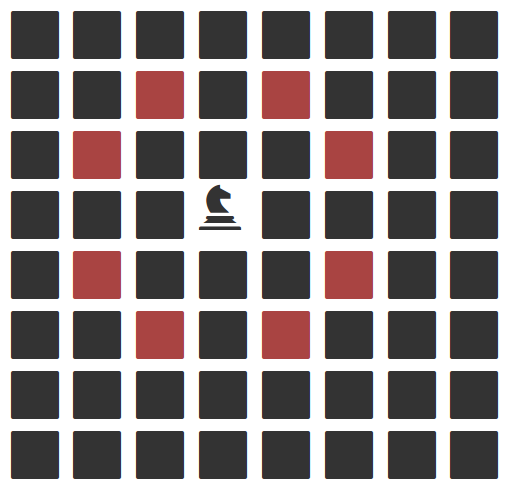
\includegraphics[scale=0.4]{imagenes/ej3/unCaballo.png}
 	\caption{Casillas que \emph{ataca} un caballo}
   \end{center}
 \end{figure}

\begin{figure}[h!] 
\centering
\begin{minipage}[t]{.45\textwidth}
\begin{center}
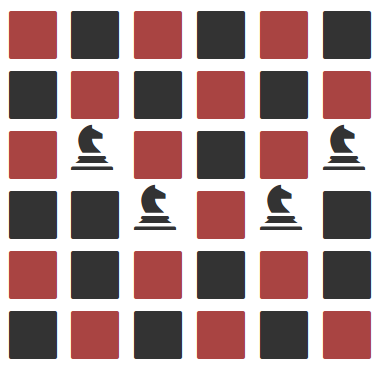
\includegraphics[width=.8\linewidth]{imagenes/ej3/6x6init.png} % primera imagen colocada a la izquierda
	\caption{As\'i se ver\'ia, un tablero dado un posible estado inicial}
\end{center}
\end{minipage}
\hfill
\begin{minipage}[t]{.45\textwidth}
\begin{center}
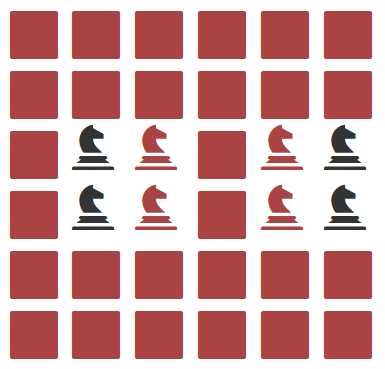
\includegraphics[width=.8\linewidth]{imagenes/ej3/6x6optima.png} % segunda imagen colocada a la derecha 
\caption{Una de las soluciones \'optimas donde se le agregan 4 caballos}
\end{center}
\end{minipage}
\hfill
%\caption{figure 1 & 2}
\end{figure}

\newpage

\subsection{Resoluci\'on propuesta y justificaci\'on}
Para la resoluci\'on de este ejercicio, se ped\'ia un algoritmo de backtracking. Es decir que el algortimo debe, a partir de una subsoluci\'on del problema, fijarse si es soluci\'on y hacer algo  al respecto con ella, o bien, si es una subsoluci\'on v\'alida, para cada elemento que se pueda agregar a la subsoluci\'on, agregarlo y repetir el proceso, o en el \'ultimo caso, si se llega a una soluci\'on no v\'alida, volver hacia atr\'as y tomar una decisi\'on adecuada.\\

Bajo el contexto de un algoritmo de Backtracking se divisan a las distintas estrategias para resolver un determinado problema como distintos caminos desde la raiz hasta una hoja dentro de un \'arbol de decisiones. En nuestro caso, cada camino va a representar cada una de las distribuciones posibles de fichas \emph{caballo} en las casillas marcadas como \emph{vac\'ias} al comienzo de la ejecuci\'on.\\

Vamos a recorrer desde la rama que no ubica ninguna pieza de caballo, hasta la que ubica caballos en todas las posiciones vac\'ias, secuencialmente.\\

Cuando llegamos al final de cada camino (una hoja) no tenemos asegurado haber \emph{cubierto} el tablero, es decir no todas las ramas van a ser soluci\'on. Pero si lo es, debemos comparar con las soluciones encontradas anteriormente, preservando siempre la que utiliz\'o una menor cantidad de fichas.\\

Habiendo recorrido todo el \'arbol, nos aseguramos de encontrar alguna soluci\'on. En particular, la \'optima o una entre las \'optimas, si hubiera m\'as de una. Esto implica que el algortimo debe revisar un (muy) extenso \'arbol de posibilidades, donde una decisi\'on es agregar o no un caballo en la posici\'on $i, j$ del tablero para todo $i, j$ dentro del rango del mismo. \\

Posterior a esto se ped\'ia pensar e implementar una serie de podas y estrategias para no recorrer todo el \'arbol, sino mirarlo inteligentemente y as\'i reducir los tiempos de ejecuci\'on.\\

Para inicializar la b\'usqueda, necesitamos guardar una soluci\'on del tablero que sea m\'axima en la cantidad de caballos agregados. Esta es, particularmente, llenar el tablero.\\

Luego el algortimo es muy sencillo, pregunta cu\'antos caballos hace falta agregar para cubrir el tablero si en la posici\'on $i, j$ agrega un caballo (recursivamente llena todo el tablero) y lo compara con la respuesta de no agregarlo, guardando en el contenedor de soluciones antes mencionado, la soluci\'on m\'as \'optima hasta ese momento.\\

El algoritmo resuelve el ejercicio planteado porque efectivamente recorre todo el \'arbol de soluciones y se queda con alguna de las \'optimas (o la \'optima si hubiera una sola).\\

\newpage

\subsection{An\'alisis de la complejidad}
El algoritmo tiene una complejidad inicial de $O(n^{2})$ (siendo \emph{n} la dimensi\'on del tablero) porque crea un primer vector de soluci\'on \'optima (el cual funcionar\'a como acumulador) con ``agregar todos los caballos posibles al tablero''.\\

Conitnuando este algoritmo, hay que tener en cuenta dos situaciones.\\

\textbf{Primera Situaci\'on: }

El tablero pasado como par\'ametro de entrada se encuentra cubierto completamente con las fichas existentes.\\

Nuestro algoritmo s\'olo debe chequear que el tablero este cubierto. Lo realiza en tiempo $O(n^{2})$, dado que debe recorrer la matriz donde est\'a almacenado el tablero, posici\'on por posici\'on.\\

Que sumado a la complejidad anterior da como resultado $O(n^{2})$\\

\textbf{Segunda Situaci\'on: }

El tablero pasado como par\'ametro de entrada \emph{no} se encuentra cubierto completamente con las fichas existentes.\\

Es en este caso donde se comienza a trabajar con el \emph{Backtracking}. La primer resoluci\'on llevada a cabo fue aplicar ``fuerza bruta''. Esto consisti\'o en recorrer por completo el \'arbol de soluciones y devolver una que fuera \'optima. Para ello, en cada posici\'on sin caballos, debemos ver que pasa si tomo alguna de las dos posibles decisiones (insertar un caballo o no). Este proceso cuenta con una complejidad de $O(2^{n^{2} - k})$ siendo $k$ la cantidad de caballos preubicados. Agregar o quitar un caballo toma tiempo $O(1)$ y por cada posici\'on del tablero que est\'e libre ($n^{2} - k$ en un tablero de  $n^{2}$ casillas totales), elige entre dos opciones, agregar o no un caballo, es decir: 2x2x...x2 $O(n^{2}-k)$ veces.\\

Con el fin de disminuir los tiempos de ejecuci\'on, se pidi\'o realizar podas al \'arbol y estrategias de recorrido (determinar si vale la pena o no seguir revisando alguna rama).\\

Ninguna poda o estrategia disminuye la complejidad te\'orica exponencial estudiada, dado que el algoritmo realiza las mismas preguntas para cada posici\'on del tablero: ¿qu\'e pasa con el resto del tablero si a esta posici\'on la dejo sin caballo? y ¿qu\'e pasa con el resto del tablero si a esta posici\'on le agrego un caballo?.\\

No obstante, los tiempos de ejecuci\'on se ven radicalmente afectados (ver Secci\'on: \ref{tiempos}), esto sucede porque se poda el \'arbol de soluciones posibles que se analizan. Es decir, en un primer momento se revisaban todas las ramas, sin excepci\'on; pero aplicando podas o estrategias, descartamos caminos que ya sabemos que no nos llevar\'an a un resultado de inter\'es.\\


La poda fue la m\'as intuitiva: mientras vamos recorriendo el \'arbol contamos con una soluci\'on (preservada) que presenta \emph{k} caballos extra agregados. Si analizando otra rama nos encontramos en una posici\'on donde debemos agregar un caballo, pero la cantidad de caballos para este camino iguala a k no vamos a estar interesados en proseguir por esta rama ya que, a lo sumo, vamos a encontrar otra soluci\'on \'optima con \emph{k} caballos.\\

%si tenemos una soluci\'on con k caballos extra agregados,  y analizando otra rama llegamos a tener que necesitar agregar un caballo a una subsoluci\'on de k-1 caballos (o sea que tendr\'ia por lo menos k caballos), entonces no nos interesa seguir revis\'andola, pues tenemos una soluci\'on que es igual o m\'as \'optima con k caballos.\\

La estrategia fue preguntar, para cada posición a analizar, si agregar un caballo en dicha posici\'on cubre alguna casilla que estaba libre (incluyendo en la cual es colocada). Si no lo hace, podemos establecer que este caballo no se va a encontrar en el Conjunto Solución de esa rama, por lo que podemos descartarla.

Entonces, no solo salteamos las k posiciones de los caballos preubicados, sino que también salteamos aquellas posiciones en las cuales agregar un caballo no modifica mi estado anterior, es decir, que estar\'ian atancando casilleros que ya est\'an siendo cubiertos por otros caballos.
  
\newpage

\subsection{C\'odigo fuente}
	\begin{codesnippet}
	\begin{verbatim}
struct casillero{
    bool esCaballo;
    long int ataques;
};
	\end{verbatim}
	\end{codesnippet}

	\begin{codesnippet}
	\begin{verbatim}
struct coordenadas{
    unsigned int fila;
    unsigned int col;
};
	\end{verbatim}
	\end{codesnippet}


	\begin{codesnippet}
	\begin{verbatim}
int main(int argc, char const *argv[]){
    chrono::time_point<chrono::system_clock> start, end;
    long int cantCaballos;
    cin >> dimension;
    cin >> cantCaballos;
//Creamos un tablero sin caballos
    Tablero tablero(dimension, Vec(dimension));
    for (int i = 0; i < dimension; ++i){
        for (int j = 0; j < dimension; ++j){
            casillero actual;
            actual.esCaballo = false;
            actual.ataques = 0;
            tablero[i][j] = actual;
        }
    }
//Leemos informacion del problema
    int fila;
    int col;
    for (int i = 0; i < cantCaballos; ++i){
        cin >> fila;
        cin >> col;
//Agregamos los caballos y las posiciones a las que ataca
        tablero[fila-1][col-1].esCaballo = true;
        atacame(tablero, fila-1, col-1, 1);
    }
    start = chrono::system_clock::now();
//Aplicamos el algoritmo
    vector<coordenadas> sol = senorCaballos(tablero);
    end = chrono::system_clock::now();
//Stdout pedido
    cout << sol.size() << endl;
    for (int i = 0; i < sol.size(); ++i){
        cout << sol[i].fila+1 << " " << sol[i].col+1 << endl;
    }
    chrono::duration<double> elapsed_seconds = end-start;
    cout << "Tiempo: " << elapsed_seconds.count() << endl;
    return 0;
}
	\end{verbatim}
	\end{codesnippet}
\newpage
	\begin{codesnippet}
	\begin{verbatim}
vector<coordenadas> senorCaballos(Tablero& t){
//Creamos un vector de n*n, con n = dimension del tablero, 
//"la peor manera de cubrir un tablero es colocando un caballo en cada casillero"
    coordenadas aca;
    vector<coordenadas> optimo;
    for (int i = 0; i < dimension; ++i){
        for (int j = 0; j < dimension; ++j){
            aca.fila = i; aca.col = j;
            optimo.push_back(aca);
        }
    }
//Creamos el vector solucion
    vector<coordenadas> agregados;
    senorCaballosAux(t, 0, 0, agregados, optimo);
    return optimo;
}
	\end{verbatim}
	\end{codesnippet}

	\begin{codesnippet}
	\begin{verbatim}
void atacame(Tablero& t, int fila, int col, int ataco){
//ataco = 1 ataca, ataco = -1 desataca
    if(col-2 >= 0){
        if(fila-1 >= 0) t[fila-1][col-2].ataques += ataco;
        if(fila+1 < dimension) t[fila+1][col-2].ataques += ataco;
    }
    if(col+2 < dimension){
        if(fila-1 >= 0) t[fila-1][col+2].ataques += ataco;
        if(fila+1 < dimension) t[fila+1][col+2].ataques += ataco;
    }
    if(fila-2 >= 0){
        if(col-1 >= 0) t[fila-2][col-1].ataques += ataco;
        if(col+1 < dimension) t[fila-2][col+1].ataques += ataco;
    }
    if(fila+2 < dimension){
        if(col-1 >= 0) t[fila+2][col-1].ataques +=ataco;
        if(col+1 < dimension) t[fila+2][col+1].ataques +=ataco;
    }
}
	\end{verbatim}
	\end{codesnippet}

	\begin{codesnippet}
	\begin{verbatim}
bool chequeo(const Tablero& t){
    for (int i = 0; i < dimension; ++i){
        for (int j = 0; j < dimension; ++j){
            if(!t[i][j].esCaballo && t[i][j].ataques == 0){
                return false;
            }
        }
    }
    return true;
}
	\end{verbatim}
	\end{codesnippet}

	\begin{codesnippet}
	\begin{verbatim}
int senorCaballosAux(Tablero& t, int i, int j, vector<coordenadas>& agregados, 
vector<coordenadas>& optimo){
//si el tablero esta cubierto, dadas las podas será una solución optima, 
//la guardamos y retornamos cuantos caballos agregamos
    if(chequeo(t)){        
        optimo.assign(agregados.begin(),agregados.end());
        return optimo.size();
    }
//sino si estoy dentro del tablero
    int siAgrego, siNoAgrego;
    if(i<dimension){
//  si hay un caballo preubicado, salteo el espacio
//  si la posicion esta atacada y de agregar un caballo no cubre ninguna previamente cubierta, 
//  no es lo que busco
        if(t[i][j].esCaballo || (!sirveAgregar(t, i, j) && t[i][j].ataques > 0)){
            j++;
            if(j==dimension){
                j=0; i++;}
            return senorCaballosAux(t, i, j, agregados, optimo);
        }
//  sino backtracking
        else{
//      si tengo un optimo de k caballos, y llegue a una subsolucion de k-1 caballos que aun 
//      no cubre todo el tablero, no es lo que busco
            if(agregados.size() >= optimo.size()-1)
                return -1;
//      PRUEBO SIN AGREGAR UN CABALLO
//      si no termine la fila
            if(j<dimension-1)
                siNoAgrego = senorCaballosAux(t, i, j+1, agregados, optimo);
//      si tengo que cambiar de fila
            else
                siNoAgrego = senorCaballosAux(t, i+1, 0, agregados, optimo);
//      PRUEBO AGREGANDO UN CABALLO
            t[i][j].esCaballo = true;
            atacame(t, i, j, 1);
            coordenadas aca; aca.fila = i; aca.col = j;
//      lo agrego a la posible solucion
            agregados.push_back(aca);
//      si no termine la fila
            if(j<dimension-1)
                siAgrego = senorCaballosAux(t, i, j+1, agregados, optimo);
//      si tengo que cambiar de fila
            else
                siAgrego = senorCaballosAux(t, i+1, 0, agregados, optimo);
//      RESTAURO el tablero y el vector con los caballos agregados
            t[i][j].esCaballo = false;
            atacame(t, i, j, -1);
            agregados.pop_back();
        }
//  si no tienen solucion agregando y sin agregar, devuelvo que no hay solucion
        if(siAgrego == -1 && siNoAgrego == -1)
            return -1;
        if(siNoAgrego==-1 || siAgrego < siNoAgrego)
            return siAgrego;
        return siNoAgrego;
    }
//sino devuelvo que no hay solucion
    return -1;
}
	\end{verbatim}
	\end{codesnippet}

\newpage

	\begin{codesnippet}
	\begin{verbatim}
bool sirveAgregar(const Tablero& t, int fila, int col){
    if(col-2 >= 0){
        if(fila-1 >= 0 && t[fila-1][col-2].ataques == 0 && !(t[fila-1][col-2].esCaballo))
            return true;
        if(fila+1 < dimension && t[fila+1][col-2].ataques == 0 && !(t[fila+1][col-2].esCaballo))
            return true;
    }
    if(col+2 < dimension){
        if(fila-1 >= 0 && t[fila-1][col+2].ataques == 0 && !(t[fila-1][col+2].esCaballo))
            return true;
        if(fila+1 < dimension && t[fila+1][col+2].ataques == 0 && !(t[fila+1][col+2].esCaballo)) 
            return true;
    }
    if(fila-2 >= 0){
        if(col-1 >= 0 && t[fila-2][col-1].ataques == 0 && !(t[fila-2][col-1].esCaballo)) 
            return true;
        if(col+1 < dimension && t[fila-2][col+1].ataques == 0 && !(t[fila-2][col+1].esCaballo))
            return true;
    }
    if(fila+2 < dimension){
        if(col-1 >= 0 && t[fila+2][col-1].ataques == 0 && !(t[fila+2][col-1].esCaballo)) 
            return true;
        if(col+1 < dimension && t[fila+2][col+1].ataques == 0 && !(t[fila+2][col+1].esCaballo)) 
            return true;
    }
    return false;
}
	\end{verbatim}
	\end{codesnippet}
	
		\begin{codesnippet}
	\begin{verbatim}
void imprimir(const Tablero& tablero){
    for (int i = 0; i < dimension; ++i){
        for (int j = 0; j < dimension; ++j){
            cout << tablero[i][j].esCaballo << "(" << tablero[i][j].ataques << ") ";
        }
        cout << endl << endl;    
        }
    }
	\end{verbatim}
	\end{codesnippet}

\newpage
\subsection{Experimentaci\'on}

\subsubsection{Constrastaci\'on Emp\'irica de la complejidad}\label{tiempos}

Primero analizaremos el caso en que los tableros vienen cubiertos como entrada al problema. Lo haremos ejecutando el algoritmo sin ninguna mejora, ya que s\'olo debe ejecutar un chequeo sobre el Tablero para ver si se encuentra cubierto y devolver que no es necesario agregar ning\'un caballo.

 \begin{figure}[h!]
   \begin{center}
	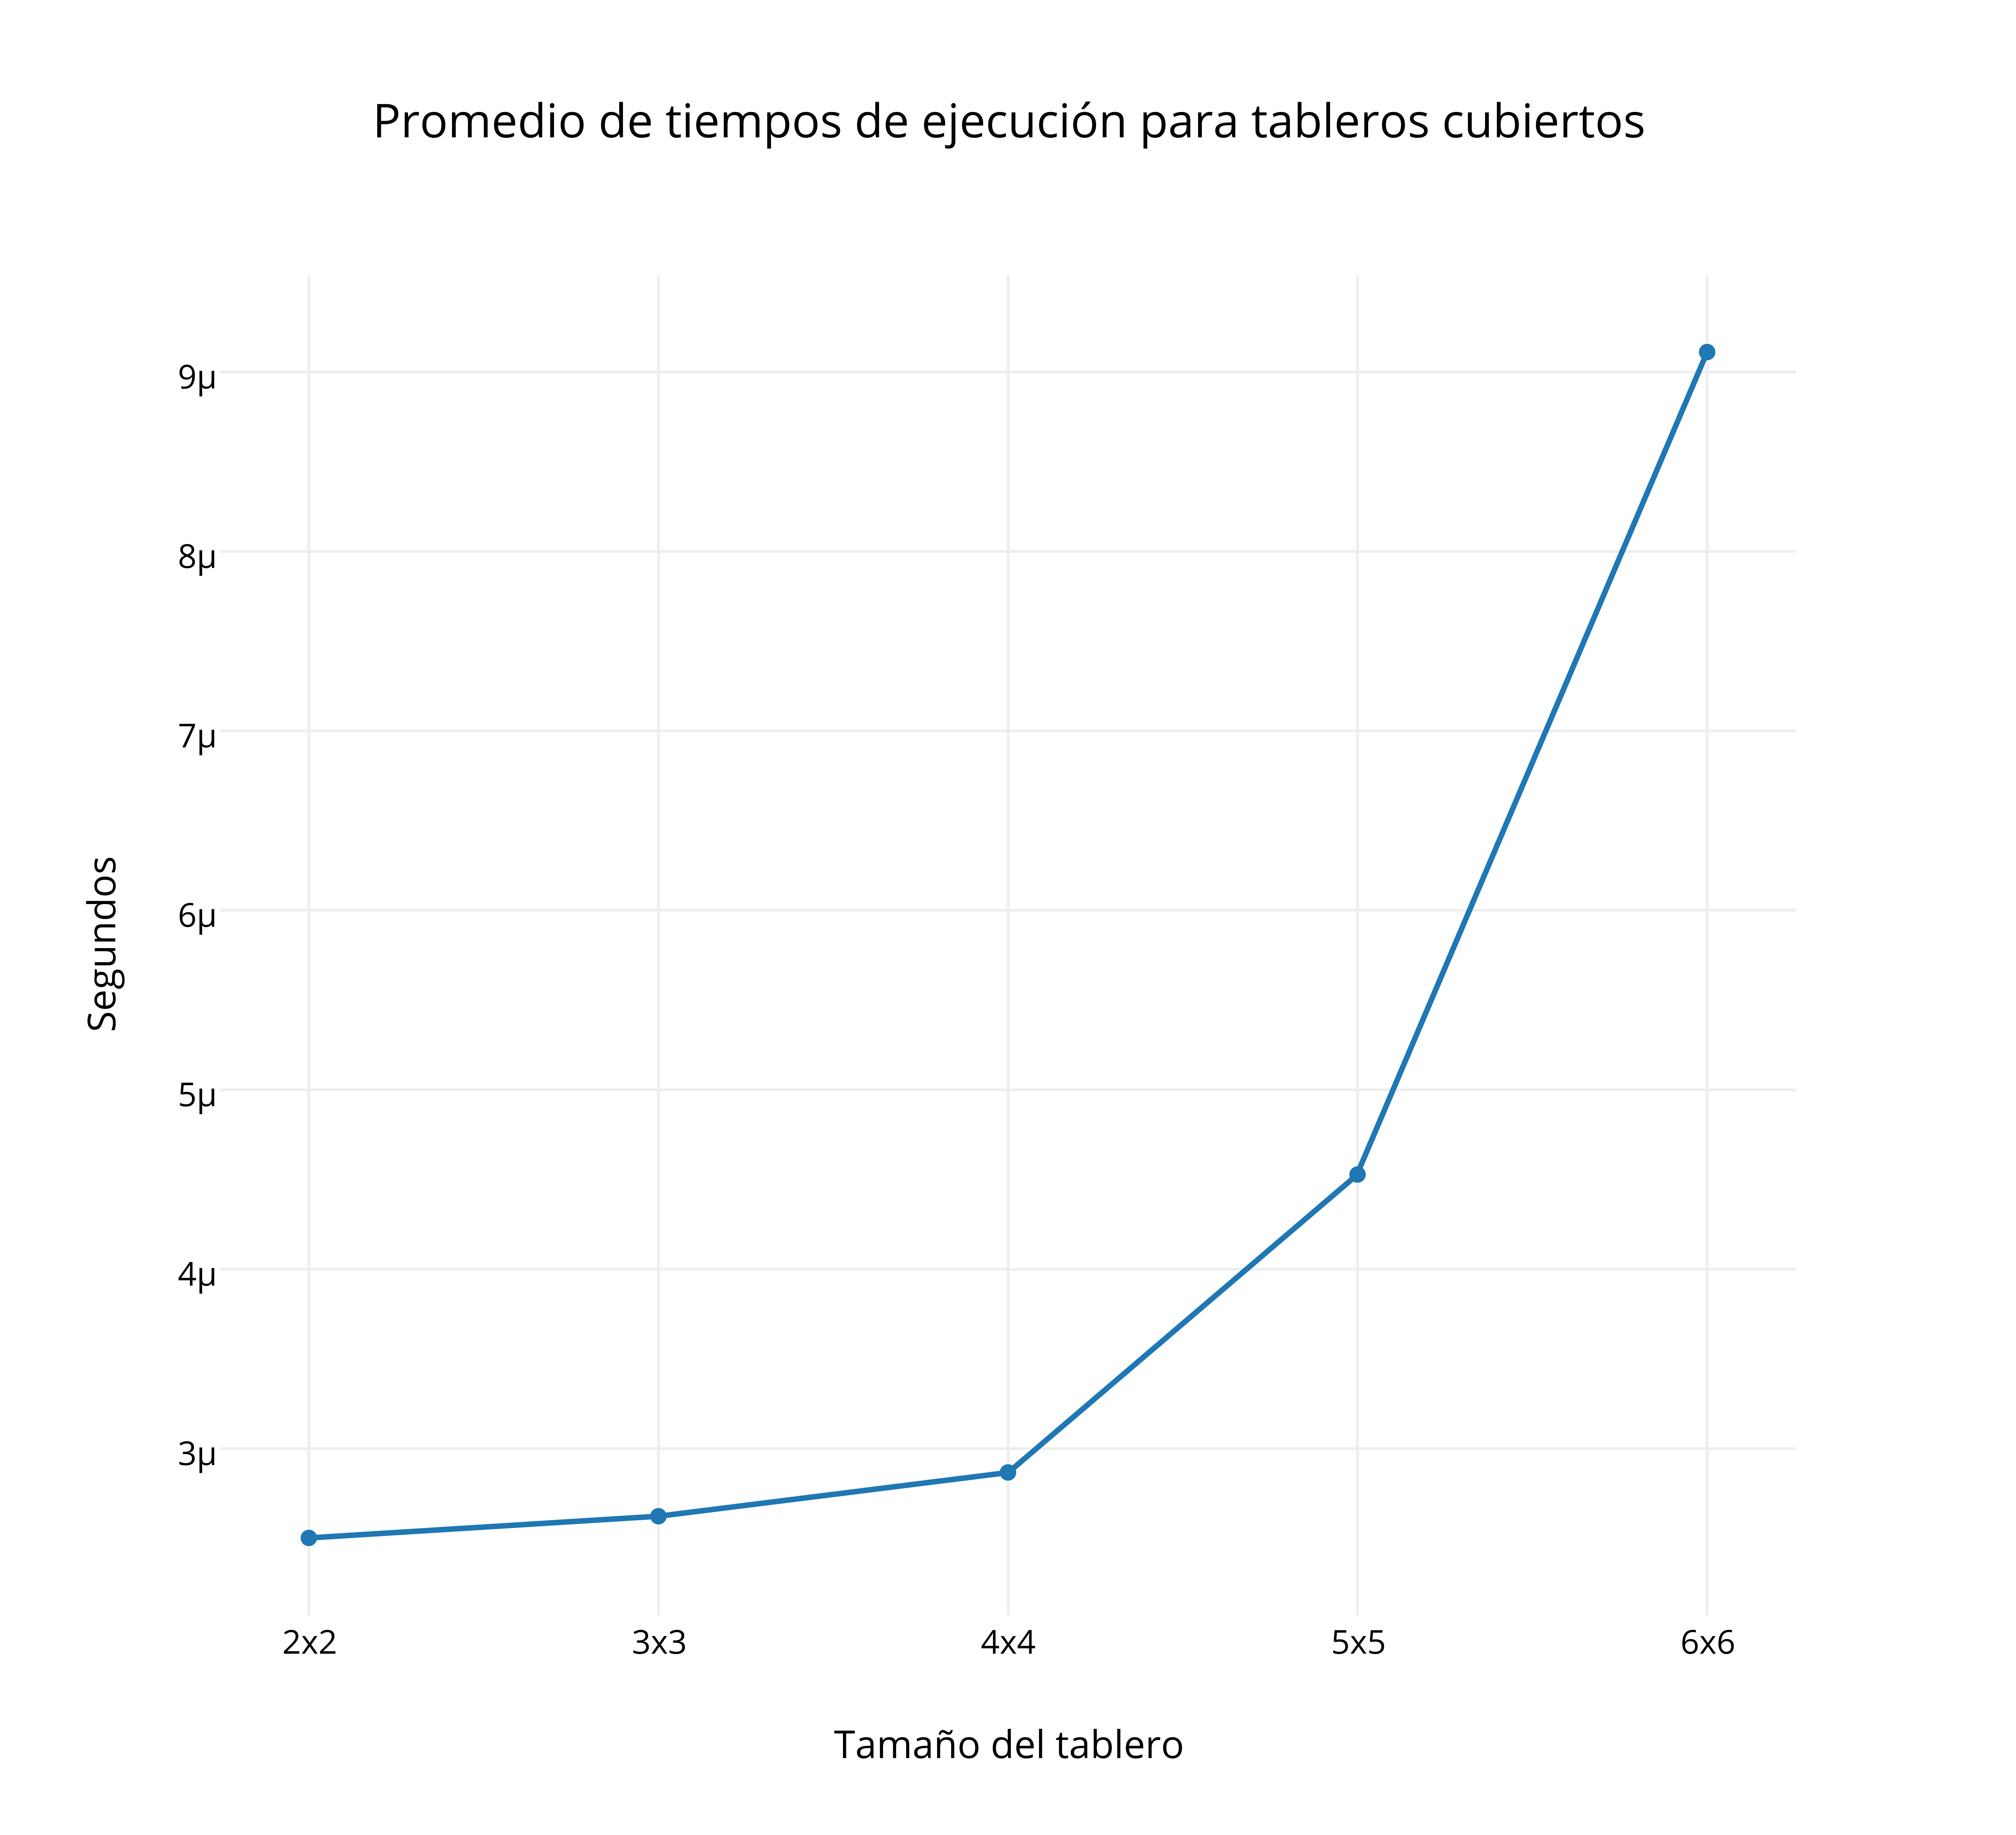
\includegraphics[scale=0.3]{../src/ej3/Mediciones/cubiertos/PromedioInforme.png} 
   \end{center}
 \end{figure}

Como se en ve en el gr\'afico, para tableros de mayor dimensi\'on, se incrementan los tiempos de ejecuci\'on. Estos aumentos aparentan seguir una curva, que en principio parece la estimada en el an\'alisis de complejidad de $O(n^{2})$.\\

%\newpage
%Dividimos por n las muestras obtenidas anteriormente (si la curva era la de $n^{2}$ entonces deber\'iamos obterner una recta) y dibujamos el siguiente gr\'afico:\\


%\textcolor{blue}{cambiar los graficos a los que correspondan!}

% \begin{figure}[h!]
%   \begin{center}
%	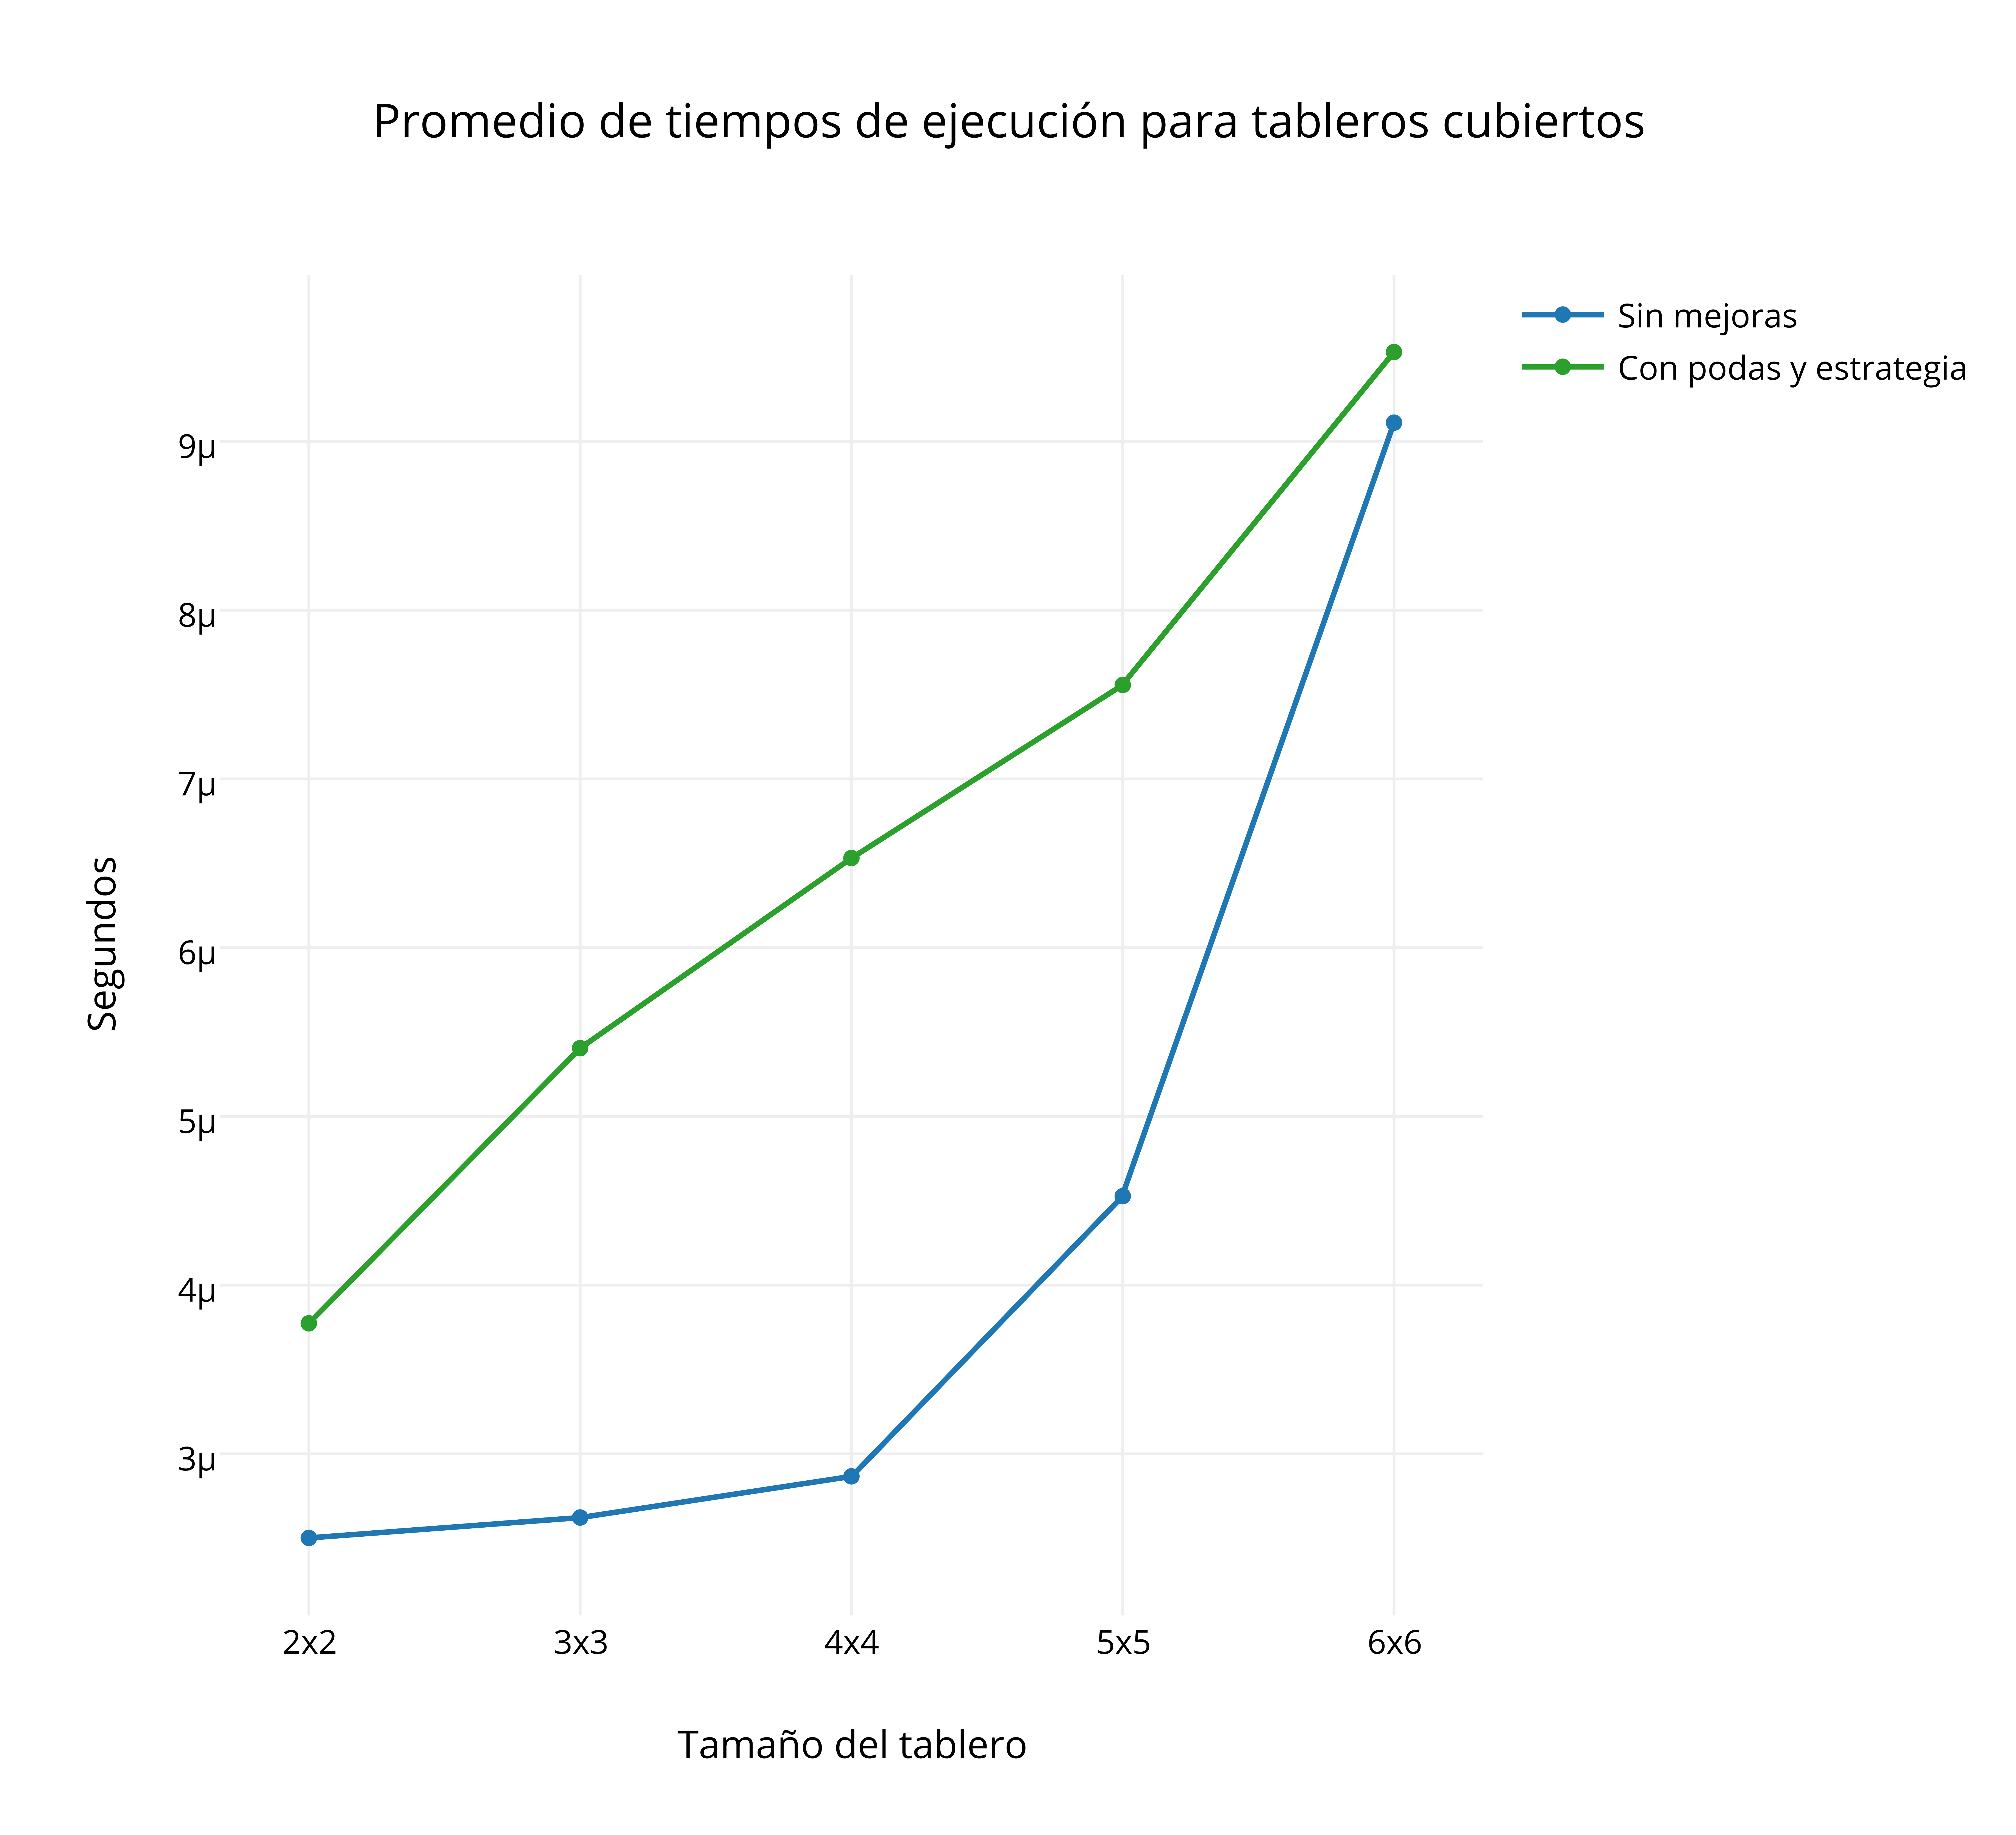
\includegraphics[scale=0.3]{../src/ej3/Mediciones/cubiertos/Promedio.png} 
%   \end{center}
% \end{figure}

%Que es una recta como esper\'abamos. En base a esto podemos concluir que la complejidad de nuestro algoritmo para tableros cubiertos demuestra también ser $O(n^{2})$.\\
\newpage

En segundo lugar vamos a ver qué sucede con los tiempos de ejecuci\'on para tableros con 0, 2 y 4 caballos preubicados, para distintos tama\~nos de tablero. Cada gr\'afico corresponde a los tiempos de ejecuci\'on del algoritmo bruto, con poda, con estrategia y con ambas situaciones a la vez para las distintas cantidades de caballos preubicados.

\underline{Nota}: para los tableros de 6x6 no tomamos mediciones en el caso de sin poda y solo estrategia porque resultaban demasiado altos.\\

\textbf{{\Large Tablero vacío}}

 \begin{figure}[h!]
   \begin{center}
   \includegraphics[scale=0.3]{../src/ej3/Mediciones/vacios/promedios1.png}
   \end{center}
 \end{figure}

Este gr\'afico muestra que a medida que aumenta el tama\~no del tablero, los tiempos aumentan. No obstante, en los tableros más chicos no se puede apreciar una diferencia significativa en cuanto a sus mediciones de tiempo. Por este motivo, haremos zoom al gr\'afico.
\newpage
 \begin{figure}[h!]
   \begin{center}
   \includegraphics[scale=0.18]{../src/ej3/Mediciones/vacios/promedios2.png}
   \end{center}
 \end{figure}

A\'un m\'as zoom...

 \begin{figure}[h!]
   \begin{center}
   \includegraphics[scale=0.18]{../src/ej3/Mediciones/vacios/promedios3.png}
   \end{center}
 \end{figure}
\newpage

Como era de esperar, el algoritmo que realiza el \emph{Backtracking completo} es el que tarda más tiempo en ejecutarse, para cualquier tamaño de tablero.\\

Adem\'as podemos ver que aplicar la estrategia (solamente) es menos eficiente que podar el árbol ya que sus mediciones de tiempo se preservan por encima de las dos curvas restantes.\\

Al momento de comparar los dos casos con podas sucede que para los tableros más pequeños las mediciones de tiempo oscilan entre sí. Esto se debe a que para tableros chicos, calcular si agregar un caballo es una buena idea o no (que es el procedimiento que se lleva a cabo en la estrategia) carece de sentido ya que hay poca probabilidad de que un caballo ataque otras posiciones del tablero que no esten cubiertas. En la mayoría de los casos, va a ser mejor agregar un caballo y después ver que pasa.

Pero al aumentar el n, los tiempos de ejecución de realizar podas sin estrategia siempre son mayores. En estos casos lo que ocurre es que llevar a cabo nuestra estrategia conviene ya que se eliminan muchas ramas del árbol de un sólo paso.

\newpage

\textbf{{\Large Tablero con dos caballos iniciales}}
 \begin{figure}[h!]
   \begin{center}
   	\includegraphics[scale=0.3]{../src/ej3/Mediciones/2caballos/promedios1.png} 
   \end{center}
 \end{figure}
   \newpage

 Haciendo zoom

 \begin{figure}[h!]
   \begin{center}
   \includegraphics[scale=0.18]{../src/ej3/Mediciones/2caballos/promedios2.png} 
   \end{center}
 \end{figure}
 
A\'un m\'as zoom...

 \begin{figure}[h!]
   \begin{center}
   \includegraphics[scale=0.18]{../src/ej3/Mediciones/2caballos/promedios3.png} 
   \end{center}
 \end{figure}
 
 \newpage
 
\textbf{{\Large Tablero con cuatro caballos iniciales}}

 \begin{figure}[h!]
   \begin{center}
   \includegraphics[scale=0.3]{../src/ej3/Mediciones/4caballos/promedios1.png} 
   \end{center}
 \end{figure}
 
Se puede apreciar que al tratar con un tablero de entrada con dos o cuatro caballos preubicados, sin estar este cubierto, los tiempos de ejecución para cada método preservan la relaci\'on analizada en el tablero vac\'io.\\

%\newpage

%\textcolor{red}{{\LARGE ARMAR EL GRÁFICO RECTIFICADO!!}}\\

%Nuestra estimación de Complejidad del algoritmo era de $O(2^{n^2}-k)$, por lo tanto decidimos aplicarle log$_2$ y dividir por $n$ a los tiempos obtenidos.\textcolor{red}{Ver que grafico va...}

%\begin{figure}[h!]
%   \begin{center}
%   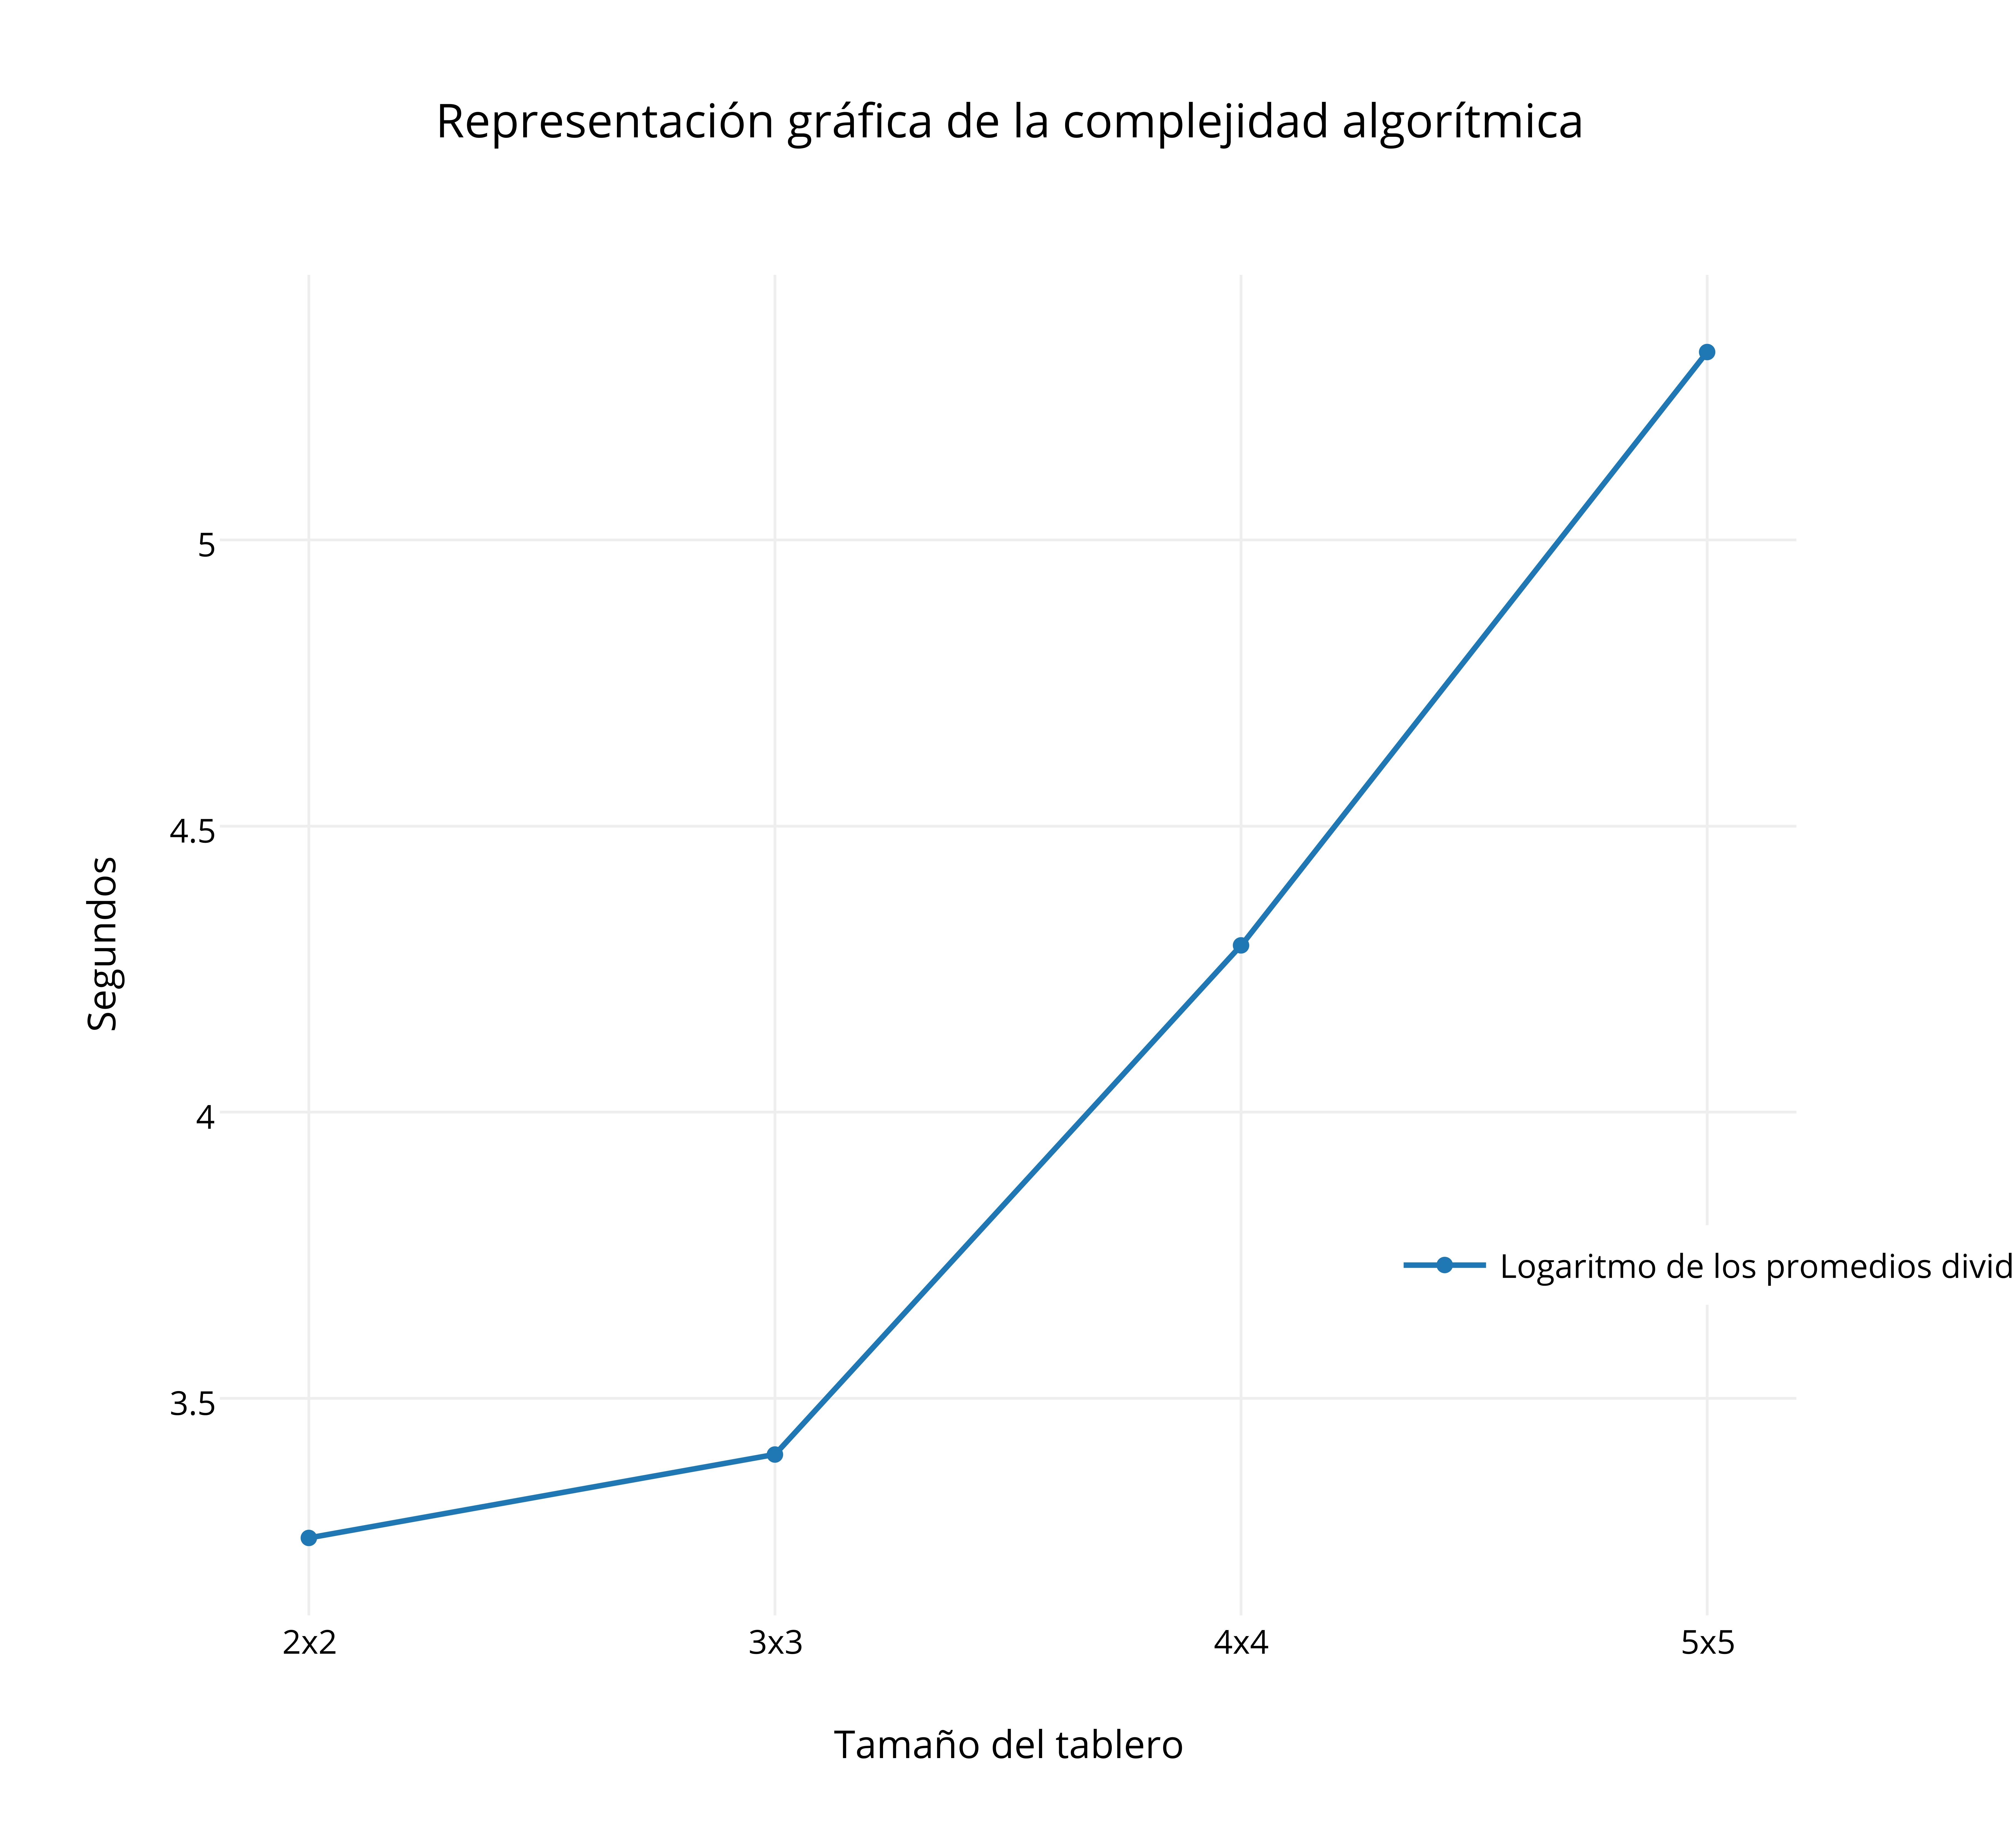
\includegraphics[scale=0.3]{../src/ej3/Mediciones/linealInf.png}
% SERA EL QUE SE LLAMA LINEAL??
%   \end{center}
% \end{figure}
 
%Se puede apreciar que el gráfico nos resultó una recta, confirmando empíricamente nuestra hipótesis sobre la complejidad.

\newpage
\subsubsection{Influencia de la cantidad de caballos preexistentes sobre los tiempos de ejecuci\'on}


Como último paso, queremos verificar si el $k$, perteneciente a nuestra cota de complejidad\\
($O(2^{n^2}-k)$), ejerce una influencia notoria en los tiempos de ejecución.

Para comprobar esto, hicimos gráficos de barras indicando cuánto tardó el algoritmo con Podas y Estrategia (a la vez) para distintos tamaños de n comparando la cantidad de caballos inicial.

\begin{figure}[h!]
   \begin{center}
\includegraphics[scale=0.3]{../src/ej3/Mediciones/Barras1.png} 
   \end{center}
 \end{figure}

\newpage
 
Haciendo zoom

\begin{figure}[h!]
   \begin{center}
\includegraphics[scale=0.173]{../src/ej3/Mediciones/Barras2.png} 
   \end{center}
 \end{figure}

Aún más zoom...

\begin{figure}[h!]
   \begin{center}
\includegraphics[scale=0.173]{../src/ej3/Mediciones/Barras3.png}
   \end{center}
 \end{figure}


 
Se puede apreciar que, independientemente del tamaño del tablero a utilizar, la relación de tiempos de ejecución es siempre la misma: el caso que menos tiempo tarda es el caso trivial (cuando el tablero está ocupado al inicio) y luego el tiempo de ejecución se incrementa acorde disminuye la cantidad de caballos preubicados.
 